\chapter[Study III: Predictive Soundscape Modelling of the Lockdowns]{Investigating Urban Soundscapes of the COVID-19 Lockdown: A predictive soundscape modelling approach}
\label{ch:lockdown}

This paper is part of a special issue on COVID-19 Pandemic Acoustic Effects.

\draft{Will update to match published version, but essentially won't need to change.}

\section*{Abstract}
 The unprecedented lockdowns due to COVID-19 in spring 2020 triggered changes in human activities in public spaces. A predictive modelling approach was developed to characterise the resulting change in the perception of the sound environment when people could not be surveyed. Building on a database of soundscape questionnaires ($N = 1,136$) and binaural recordings ($N = 687$) collected in 13 locations across London and Venice during 2019, new recordings ($N = 571$) were made in the same locations during the 2020 lockdowns. Using these 30-second-long recordings, linear multi-level models were developed to predict the soundscape pleasantness ($R^2=0.85$) and eventfulness ($R^2=0.715$) during the lockdown and compare the changes for each location. The performance was above average for comparable models. An online listening study also investigated the change in sound sources within the spaces. Results indicate:

 \begin{enumerate}
   \item human sounds were less dominant and natural sounds more dominant across all locations;
   \item contextual information is important for predicting pleasantness but not for eventfulness;
   \item in general, perception shifted towards less eventful soundscapes and to more pleasant soundscapes for previously traffic-dominated locations, but not for human- and natural-dominated locations.
 \end{enumerate}

 This study demonstrates the usefulness of predictive modelling and the importance of considering contextual information when discussing the impact of sound level reductions on the soundscape.

 \section{Introduction}
\label{sec:intro}

\subsection{Review of the impacts of COVID-19}
 \label{sec:covidReview}
 The global emergency cause by the \gls{covid19} in early 2020 required national lockdown measures across the world, primarily targeting human activity. In the United Kingdom, construction and transport were allowed to continue, but a decrease in activity was observed \citep{Hadjidemetriou2020impact}. In other countries, such as Italy, the restrictions were more severe and even included limiting people's movement to a certain radius from their place of residence \citep{Ren2020Pandemic}. The explorations in environmental acoustics of lockdown conditions across the world have revealed various degrees of impact on the acoustic environment, with researchers reporting reductions in noise levels affecting the population at the scale of urban agglomerations such as the Ruhr Area in Germany \citep{Hornberg2021Impact} and conurbations in the south of France \citep{Munoz2020Lockdown}. Impacts have also been reported at a scale of a multimillion city such as Madrid \citep{Asensio2020Changes} or Barcelona \citep{BonetSola2021Soundscape} as well as at a more local, city-centre or even public space-scale in cities such as Stockholm \citep{Rumpler2021Noise}, London \citep{Aletta2020Assessing}, Girona \citep{AlsinaPages2021Changes}, or Granada \citep{VidaManzano2021sound}. In general, these studies have demonstrated a decrease in urban noise levels and indicated a difference in the amount of decrease depending on the type of space investigated (e.g. parks, urban squares, etc.) and the type of human activity characteristic for the space, with higher reductions in places typically associated with human sounds and activities such as shopping and tourism.

 Those studies were mostly focussed around the \gls{laeq}, as well as a standardization approach to reporting subsequent changes in soundscape proposed by \citet{Asensio2020Taxonomy}. They were not able to reveal the perceptual impact of such conditions in public spaces as well because of: 1) the lack of subjective data for the exact or comparable locations in previous years; and 2) the lack of participants present in public spaces during the lockdown, hence the ability to collect soundscape data in situ. Attempts have been made to bridge this gap by using social networks to source subjective data, but this resulted in a focus on indoor conditions following the shift in the citizens' behaviour, i.e. spending more time indoors \citep{Bartalucci2021survey,Lee2021Attitudes}. \citet{GarridoCumbrera2021Perceptions} relied on an online survey deployed in England, Ireland, and Spain to explore the perceived change in natural environments in particular. They observed a consistent increase in the perceived presence of natural sounds across all major cities and rural areas respectively in these three countries. A very similar trend was observed in Argentina, also based on an online questionnaire without a listening task \citep{Maggi2021Perception}. 
 
 \citet{Munoz2020Lockdown} combined noise measurements with an online questionnaire deployed to residents, some of which were residing in the areas covered by the noise monitoring network available. The participants were asked to recall how their lockdown area sounded before and during the first lockdown in 2020 and to describe the perceived change. They observed a consistent reduction in levels, followed by the perceived reduction of transport sounds (air and road) and an increase of natural sounds, while the resulting environment was described as pleasant, calm, and peaceful. By combining field recordings and focus groups, \citet{Sakagami2020How} and \citet{Lenzi2021Soundscape} observed changes in the sound source composition and the affective quality of soundscape in a residential area in Kobe, Japan and a public space in Getxa, Spain, respectively, during the different stages of the lockdown period. Following the easing of lockdown measures, a decrease in animal and traffic sounds was observed in Kobe, while an increase in eventfulness, loudness, and presence of human sound sources, followed by a decrease in pleasantness, was shown in Getxa.

 \subsubsection{The impacts of the lockdown in London}
 \citet{Aletta2020Assessing} explored the impacts of the \gls{covid19} lockdowns on the acoustic environment in London in particular, through many short-term (30s) binaural recordings and presented an important early analysis of the changes in acoustic features during the lockdown. The data from this study form the basis for the modelling presented in this chapter; the results and analysis of \citep{Aletta2020Assessing} were performed by the author of this thesis and are reviewed in depth. 

 %NOTE: The paras and figures here are taken directly from Aletta2020 and Tong 2021, but represent the work I did on the paper. May need to check if this is fine to present it this way.
 The lockdown measures implemented in the UK to contain the spread of the SARS-CoV-2 virus were not particularly strict if compared with other countries. In general, lockdown measures involved "staying at home" recommendations, social distancing, stopping non-essential commercial activities, banning public gatherings, limiting traffic mobility and alike. Specifically, the UK Government passed the Health Protection (Coronavirus, Restrictions) (England) Regulations 2020, which were put into place at 1:00 pm on \nth{26} March 2020 \cit{Public Health England, 2020}. Under these restrictions, the public were only allowed to leave their homes once per day for essential activities and exercise. All officers and shops selling non-essential goods were told to close, gatherings of more than two people in public were banned, and individuals were advised to only interact with members of their own household. These restrictions were set to be reviewed by the Secretary of State at least once every 21 days and would continue indefinitely until they were no longer necessary to prevent the spread of infection in England. In practice the lockdown continued through the spring of 2020 and was first partially eased on the \nth{1} of June, with school children in England returning to school, but the broader lockdown continued throughout the summer \citep{Tong2021Increases}.

 Taking advantage of short-term acoustic measurements carried out in 2019 which formed the \gls{isd}, before the implementation of the lockdown measures related to \gls{covid19}, a number of urban locations were selected in London where data were available and measurements were performed again according to the same protocols to assess the extent of sound level variation achieved at each site. 

 \paragraph*{Data analysis}
 From the binaural recording datasets (both the 2019 and 2020 series), the following acoustic parameters were computed for the left and right channels and the arithmetic average was presented: \gls{laeq}, \gls{la10}, \gls{la90}. There is still no clear consensus on how to merge binaural psychoacoustic readings into single values; in the case presented in \citet{Aletta2020Assessing} an arithmetic average level was deemed to be acceptable as the interaural level difference was typically very small (less than 1 dB) \cit{27}.

 The same procedure was followed for the psychoacoustic metrics of Loudness (\gls{n5}, sone) and Sharpness (\gls{s}, acum). All parameters were computed using the ArtemiS Suite software (v11.5, HEAD acoustics GmbH). Loudness was calculated according to the ISO 532-1 standard for time-varying sounds, in a free-field, with the remaining analysis options left to their default \citep{ISO532Part1}. As recommended by the standard, in order to avoid the under-estimation of evaluated loudness which is seen when using the arithmetic average of the loudness curve, the \gls{n5} value (the 5\% percentile value of the time-dependent loudness curve) is used as the single value of loudness. Sharpness was calculated according to DIN 45692, in a free-field, with the remaining analysis options left to their default \cit{DIN45692}. It was decided to include psychoacoustic parameters as they can often provide more nuances about the perception of the acoustic environment by people, as well as offer more insights into spectral features that could reflect changes in sound sources \cit{30,31}. Considering the necessity of keeping the computational time limited in this initial study, Loudness and Sharpness were selected because they have been reported to provide a sensible representation of perceptual aspects. \cit{32}

 \begin{figure}
  %TODO: Redo these figures in python using ISD
  \label{fig:NsMapLockLAeq}
   \caption{Reproduced with permission from \citet{Aletta2020Assessing}. On the left: Sound levels distributions at the 11 London locations before and during the lockdown measures implementation; on the right: Sound levels distributions (aggregated across locations) and corresponding mean values before and during the lockdown measures implementation.}
   \centering
   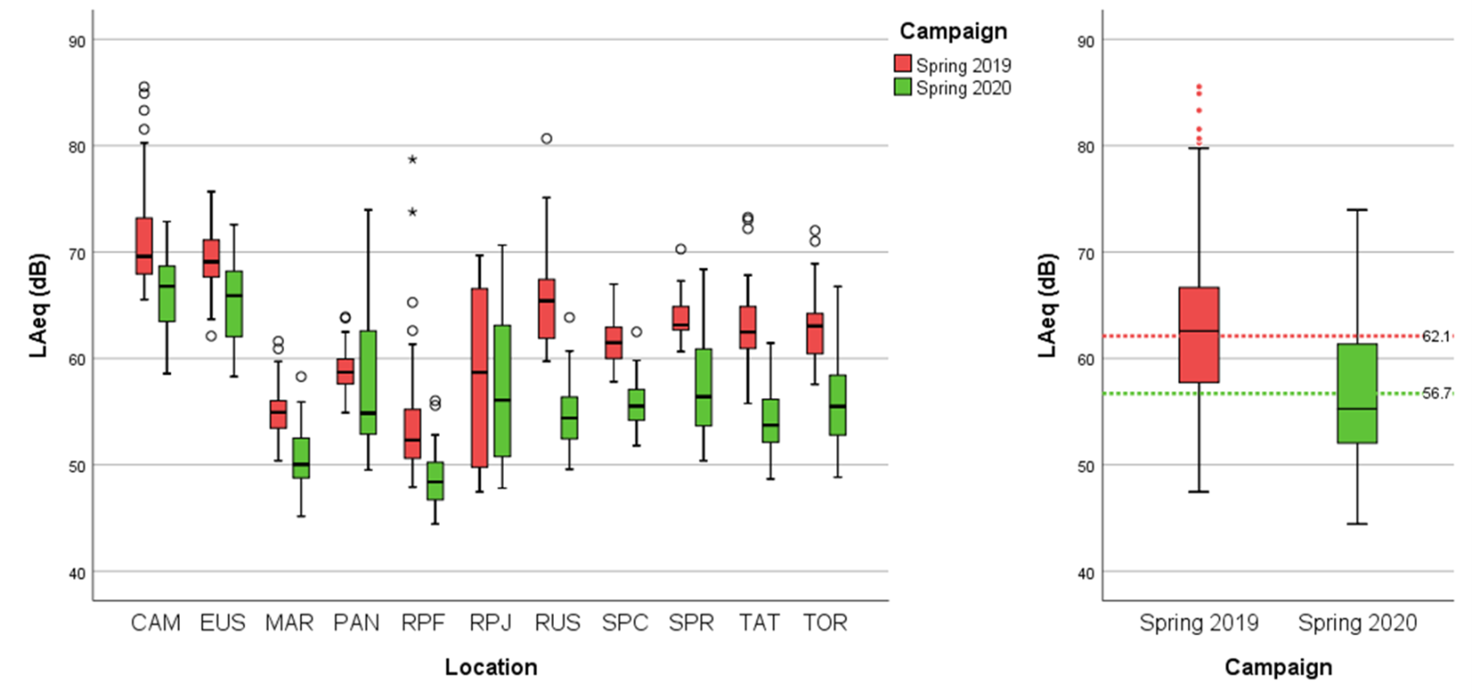
\includegraphics[width=\textwidth]{Figures/NoiseMappingLockdown Fig 1.png} 
  \end{figure}

%TODO: Discuss LAeq figure results in own wods

\begin{figure}
  \label{fig:NsMapLockN5}
  \caption{Reproduced with permission from \citet{Aletta2020Assessing}. Loudness distributions at the 11 London locations before and during the lockdown measures implementation.}
  \centering
  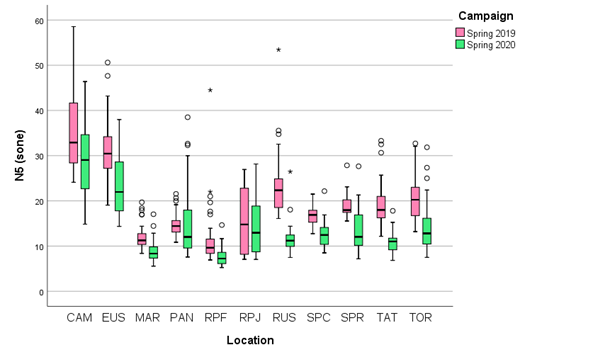
\includegraphics[width=\textwidth]{Figures/NoiseMappingLockdown Fig 4.png}
\end{figure}

%TODO: Discuss N5 figure in own words

\begin{figure}
  \label{fig:NsMapLockS}
  \caption{Reproduced with permission from \citet{Aletta2020Assessing}. Sharpness distributions at the 11 London locations before and during the lockdown measures implementation.}
  \centering
  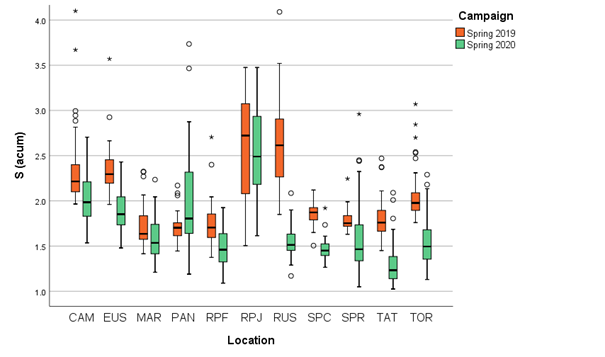
\includegraphics[width=\textwidth]{Figures/NoiseMappingLockdown Fig 5.png}
\end{figure}

%TODO: Discuss S figure in own words


\paragraph*{Effect of the urban setting on sound levels reduction}
In addition to strictly documenting the changes in the sound environment in London, the study also aimed to investigate whether the lockdown measures would result in different sound level reductions depending on the urban scenario (and its composition of sound sources). For this purpose, it was decided to define an "Area type" variable that would serve as a proxy for urban (acoustic) context: a \emph{k}-means cluster analysis was performed on the mean values of \gls{laeq}, \gls{la10}, \gls{la90}, \gls{n5}, and \gls{s} of the 2019 measurements campaign for the 11 locations, after those have been \emph{z}-score standardized to meet the algorithm criteria. The rationale was that clustering urban areas \emph{a priori} based on their "typical" acoustic climate (hence using only data from 2019) would allow us to see whether there was an association between area type and noise reduction. The algorithm was set to a three-cluster solution, based on visual inspection of the scree plot as report in Figure \ref{fig:NsMapLockScree} ("elbow method") \cit{33}. The analysis was conducted in R \cit{RStats} and figures were produced using the package factoextra \cit{factoextra}. 

\begin{figure}
  \label[]{fig:NsMapLockScree}
  \caption{Reproduced with permission from \citet{Aletta2020Assessing}. "Scree" plot used to identify the optimal number of clusters to use in the \emph{k}-means clustering algorithm where an "elbow" can be identified for a three-cluster solution.}
  \centering
  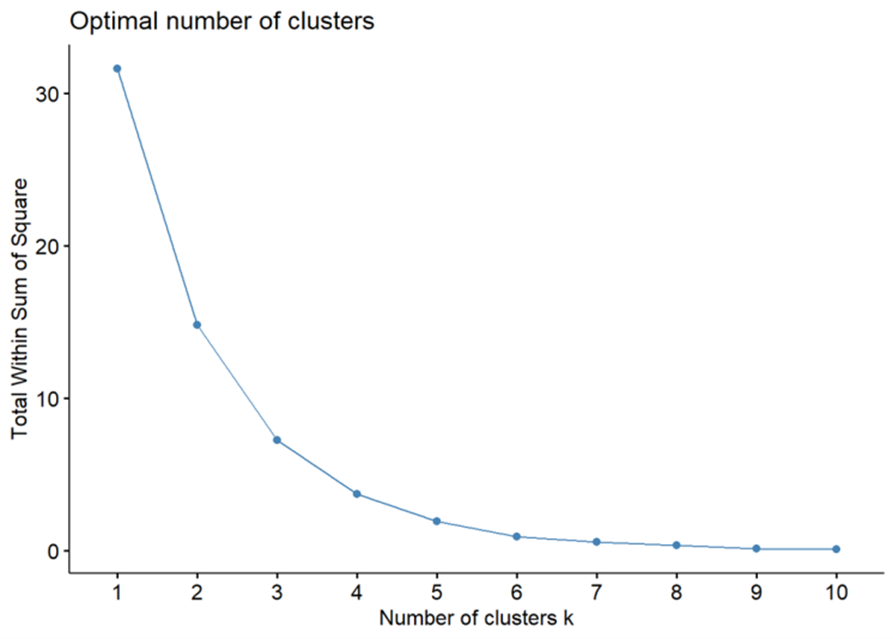
\includegraphics[width=\textwidth]{Figures/NoiseMappingLockdown Fig 6.png}
\end{figure}

Figure \ref{fig:NsMapLockBiplot} shows a plot of clustered data based on the two most relevant underlying dimensions for the three-cluster solution. Dimension 1 seems to describe a pattern related to sound level and associated metrics, whilst Dimension 2 is related to Sharpness. This is consistent with previous findings in literature where it was observed that when it comes to categorization and classification of urban acoustic environments based on objective features, most solutions are reduced to intensity- and spectral-related parameters \cit{36, 37}. 

\begin{figure}
  \label{fig:NsMapLockBiplot}
  \caption{Reproduced with permission from \citet{Aletta2020Assessing}. Di-dimensional plot for the three-cluster solution. The clusters have been labelled as: Cluster 1 -- Quiet Areas; Cluster 2 -- Active Areas; Cluster 3 -- Traffic-dominated Areas.}
  \centering
  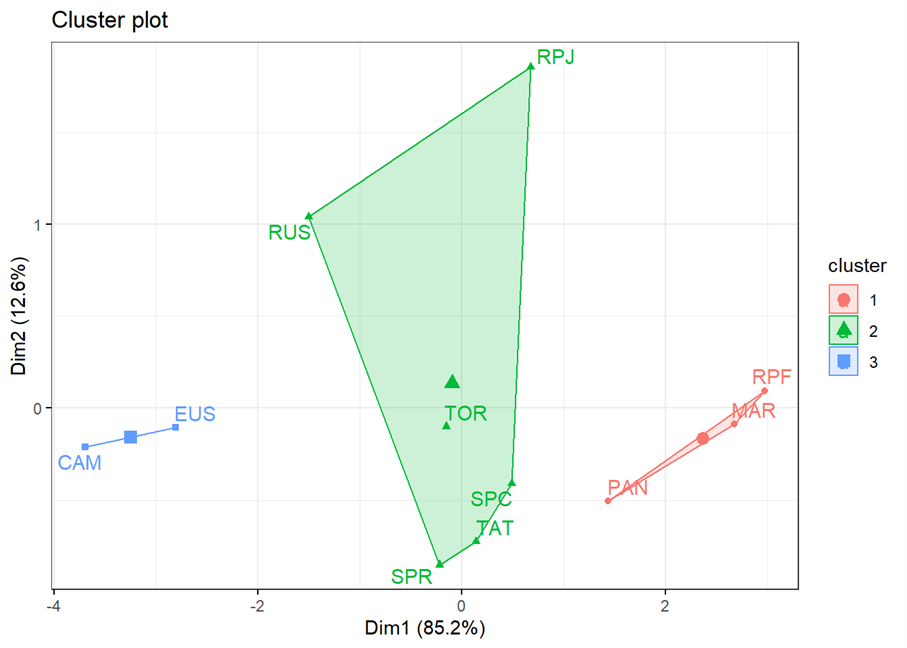
\includegraphics[width=\textwidth]{Figures/NoiseMappingLockdown Fig 7.png}
\end{figure}

Table \ref{tab:NsMapLockClust} shows the basic descriptive statistics of the psychoacoustic features for the 11 locations according to cluster membership; when combining those patters with information about dominant sound sources as derived from data from \cit{26}, the three clusters could be labelled as: \emph{Traffic-dominated areas} (locations: Camden Town, Euston Tap), \emph{Active Areas} (locations: Regents Park Japan, Russell Square, St Pauls Cross, St Pauls Row, Tate Modern, Torrington Square) and \emph{Quiet Areas} (locations: Marchmont Garden, Pancras Lock, Regents Park Fields). Traffic-dominated areas are on major roads, where traffic noise is the dominant sound source. Active areas are locations where the human activity (also combined with traffic) is the main contributor to the acoustic environment. Quiet areas are generally parks or areas with greenery that tend to have a relatively low background noise (lack of traffic sources).

When considering the mean \gls{laeq} reductions between 2019 and 2020 as a function of Area type, it can be observed that they vary across the three clusters, as shown in Figure \ref{fig:NsMapLockRedux}. The biggest reductions are for Active areas (M = 6.6 dB; SD = 3.2 dB), followed by Traffic-dominated areas (M = 4.5 dB; SD = 0.8 dB), and Quiet areas (M = 3.6 dB; SD = 1.9 dB). A possible explanation for this is that road traffic at the selected locations in London is still sustained to some extent (e.g. circulation of public transport, key workers, etc.), while the most significant variation in Active areas is possibly due to the complete lack of (non-motorized) human activity on site. The locations in the cluster labelled as Quiet areas were already not particularly noisy even before the lockdown, thus the small changes observed are probably once again due to the absence of people.

%TODO: Reproduce the table from Aletta2020
\begin{table}
  \label[]{tab:NsMapLockClust}
  \caption{Reproduced with permission from \citet{Aletta2020Assessing}. Descriptive statistics of the psychoacoustic metrics for the three identified clusters.}
  \centering
  
\end{table}

\begin{figure}
  \label[]{fig:NsMapLockRedux}
  \caption{Reproduced with permission from \citet{Aletta2020Assessing}. Mean A-weighted equivalent sound level reductions between the pre- and during-lockdown conditions as a function of cluster membership (i.e. Area type). }
  \centering
  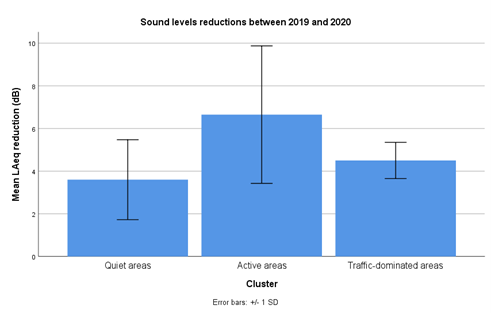
\includegraphics[width=\textwidth]{Figures/NoiseMappingLockdown Fig 8.png}
\end{figure}


 This study revealed that average reductions in the various locations considered ranged from 10.7 dB (\gls{laeq}) to 1.2 dB, with an overall average reduction of 5.4 dB. This metric-reporting focussed approach left the following research questions unanswered:
 \begin{enumerate}
   \item How would people have perceived these spaces as a result of this change in acoustic environment? (RQ1)
   \item Would these sound level reductions result in improvements to the soundscape of the spaces? (RQ2)
 \end{enumerate}

 The \nth{1} research question (RQ1), addressing the perceptual effect of the change in urban soundscape induced by the lockdowns, can be further broken down into the following questions:

 \begin{itemize}
   \item How was the sound source composition influenced by the change?
   \item How would the affective response to the acoustic environment in lockdowns change?
   \item Could this demonstrate the effect of human activities on the perception of an acoustic environment in general?
 \end{itemize}


 \subsection{Review of predictive modelling}
 These questions arise out of the soundscape approach, which is characterised by prioritising the perceptual effect of an acoustic environment by taking into account the interaction of sound sources, context, and the person perceiving it \citep{ISO12913Part1,Truax1999Handbook}, bringing together objective and subjective factors. The soundscape approach to noise mitigation and management is being recognised as a response to arising environmental requirements on noise pollution and sustainability, such as the regulation of quiet areas in Europe \citep{EEA2020Environmental, Aletta2018Towards,Radicchi2021Sound}. This has been further formalised in \citet{ISO12913Part2} via the adoption of the circumplex model of soundscape \citep{Axelsson2010principal}, in which the perception of a soundscape can be described in terms of its pleasantness and eventfulness, as one of the standard methods of soundscape assessment.

 Soundscape research is therefore traditionally rooted in environmental acoustics and environmental psychology, typically dealing with outdoor spaces \citep{Torresin2020Indoor} and urban open spaces, where parks and squares are often used as case study sites \citep{Kang2007Urban}. A soundscape assessment typically requires people to be surveyed but the presence of people at a location influences assessment \citep{Aletta2018Towards} and 'quiet places' usually require low numbers of users to remain quiet, which limits the possibility of an assessment. Even in a crowded public space, soundscape surveys are demanding as they require significant resources to carry out at scale, limiting their widespread application \citep{Mitchell2020Soundscape}. Therefore, a need for a predictive model arises to overcome this limitation and improve the implementation of the soundscape approach into everyday planning and management practices.

 According to a recent review of predictive soundscape models from \citet{Lionello2020systematic}, the degree of employing auditory and non-auditory factors in soundscape prediction varies with some studies relying on contextual \citep{Kajihara2017Imaginary}, personal/demographic \citep{Erfanian2021Psychological,Tarlao2020Investigating} or social media \citep{Aiello2016Chatty} data entirely to predict and generate soundscape features. Some methods also incorporate perceptually-derived features, such as subjective sound level and visual pleasantness as predictors \citep{Lionello2020systematic}. In general, these methods which incorporate perceptually-derived inputs achieve better accuracy rates than those which don't, however this information must also be obtained from people via a survey and therefore are unsuitable for predictive modelling where surveys are not possible. For example, \citet{Ricciardi2015Sound} proposed two models based on data collected from a smartphone application to predict urban sound quality indicators based on linear regressions. The first model which incorporated perceptually-derived input features (visual quality and familiarity) achieved an $R^2$ of 0.72, while a second model without these features achieved an $R^2$ of 0.58. This indicates the necessity for considering and accounting for the influence which contextual factors in a space have on the relationship between the sound environment itself and the listener's perception of it (i.e. the soundscape) while also highlighting the challenges associated with a predictive model which depends only on measurable features.

 Therefore, a third research question arises: what are the key features needed for a soundscape prediction model based on comprehensive acoustic on site measurements to be used for assessing locations with low social presence or in situations where conducting surveys is impractical (RQ3)?

\section{Materials and Methods}

 This study was conducted via initial onsite data collection campaigns in Central London and Venice in 2019 before the outbreak of \gls{covid19} as part of the \gls{ssid} project \citep{Mitchell2020Soundscape} and in 2020 during the strictest part of the lockdowns \citep{Aletta2020Assessing}, including objective acoustic data (2019 and 2020) and subjective responses (2019 only). The full in situ dataset, as described in this section, has been made publicly available as "The International Soundscape Database (V0.2.1)" on Zenodo (\url{https://zenodo.org/record/5654747}) \citep{Mitchell2021International}.
 
 Using both 2019 and 2020 binaural recordings, an online listening experiment was conducted to provide an understanding about the change in sound source composition. The 2019 onsite questionnaire data were used to define the dominant sound source at each location as a starting point for interpreting the soundscape change. A predictive model was developed to reveal the change in the perceived pleasantness and eventfulness using objective acoustic data and location to predict subjective responses. Although the initial (2019) dataset contains additional locations (specifically, in Spain, the Netherlands, and China), due to the nature of this study as a reaction to the strict movement and activity restrictions, the sites which could be included in the lockdown (2020) measurement campaigns were limited to locations where staff and equipment had access and where recordings could be undertaken during the spring of 2020.

 The sites were selected to provide a mixture of sizes and uses, varying in typology ranging from paved squares to small and large parks to waterside spaces across both cities. Throughout the text they are indexed via a LocationID based on the location's name (e.g. CamdenTown, SanMarco), while a more in-depth overview of each is given in supplementary files. %NOTE: Will need to adjust this within thesis.
 London is taken as an example of a large, typically noisy city while the Venice sample provides a unique look at spaces with typically very high human activity levels and no road traffic activity. In particular, the 2019 Venice surveys were taken to coincide with the yearly Carnevale festival in order to capture its distinct soundscape.

\citet{ISO12913Part2} was consulted for reporting on soundscape data. A detailed description of the 2019 survey campaigns in featured through the paper and in the public database. This study was approved by departmental UCL IEDE Ethics Committee on \nth{17} July 2018 for onsite data collection and on the \nth{2} of June 2020 for the online listening experiment and is conducted in adherence to the ethical requirements of the Declaration of Helsinki \citep{WMA2013World}.

 \subsection{Onsite data: Questionnaires, binaural measurements, and recordings}
   %FIXME: Likely will not need this within thesis.
   The initial onsite data collection featured both questionnaire data collected from the general public and acoustic measurements, conducted across thirteen urban locations (in London $N=11$, in Venice $N=2$) between the \nth{28} of February and the \nth{21} of June 2019, with additional sessions in July and October 2019. Although the total survey period in 2019 extended over several seasons, the surveys at any individual location did not extend over seasons with different occupancy patterns. A total of 1,318 questionnaire responses were collected from the general population across the measurement points during 1 -- 3 hour-long campaigns in both cities in 2019, accompanied by 693 approximately 30-second long 24-bit 44.1 kHz binaural recordings. After data cleaning, each of the 13 locations was characterised by between 14 to 80 recordings and between 24 to 147 questionnaire responses. Mean age of the participants was 33.9, with a standard deviation of 14.57 (45\% male, 53.8\% female, 0.4\% non-conforming, 0.9\% prefer-not-to-say).

   Although recent results from both \citet{Tarlao2020Investigating} and \citet{Erfanian2021Psychological} indicate the important influence of personal and demographic factors -- in particular age and gender -- on soundscape perception, these factors were not included as potential features in the modelling process. Given the nature of this study as addressing a scenario when people could not be surveyed, no additional demographic information is available in the lockdown case to be fed into the model and is therefore not useful to include for the development and application of this specific predictive model. This information is reported throughout the study simply to provide further context to the data collection.

   The subsequent measurement campaign in 2020 mimicked the binaural recording strategy applied in the initial campaign and was performed between the \nth{6} and the \nth{25} of April 2020 in both cities, this time excluding the questionnaire. An additional 571 binaural recordings were collected on site in 2020.

   \subsubsection{Data collection}
   %FIXME: Probably don't need this section in thesis either.
   The 2019 data collection was performed across all the locations using the protocol based on the Method A of the ISO/TS 12913-2:2018 \citep{ISO12913Part2}, as described in \citep{Aletta2020Assessing,Mitchell2020Soundscape}, collected either via handheld tablets or paper copies of the questionnaire. The full questionnaire and data collection procedure are given in \citet{Mitchell2020Soundscape}, however the key parts used for this study are those addressing sound source dominance and \gls{paq}.
   %NOTE: Skipping next section since it's detailed earlier in thesis.

   %NOTE: add a section to the methods about the projection. Heavy reference to / pulling from Lionello 2020 and JASA-EL paper.
   In order to simplify the results and allow for modelling the responses as continuous values, the 8 \gls{paq}s undergo a trigonometric projection to reduce them onto the two primary dimensions of pleasant and eventful, according to the procedure outlined in Part 3 of the ISO 12913 series \citep{ISO12913Part3}. In order to distinguish the projected values from the Likert-scale \gls{paq} responses, the projected values will be referred to as \gls{isopl} and \gls{isoev} and can be considered to form an x-y coordinate point (x = \gls{isopl}, y = \gls{isoev}) as explained in detail in \citet{Lionello2021Introducing}.

   %NOTE: Skipping paragraph on binaural recording info

   \subsubsection{Data cleaning}
   %TODO: Move and expand this data cleaning section to the methods section
   The cleaning of the samples was conducted using the ArtemiS SUITE 11. The researcher discarded or cropped whole recordings, or its parts affected by wind gusts or containing noises and speech generated by the recording operator by accident or for the purpose of explaining the questionnaire to a participant. This resulted in 1,291 binaural recordings which were then processed further, as described in Section \ref{sec:analyses}. Psychoacoustic analyses are shown in the publicly available database.

   In order to maintain data quality and exclude cases where respondents either clearly did not understand the \gls{paq} adjectives or intentionally misrepresented their answers, surveys for which the same response was given for every \gls{paq} (e.g. 'Strongly agree' to all 8 attributes) were excluded prior to calculating the ISO projected values. This is justified as no reasonable respondent who understood the questions would answer that they 'strongly agree' that a soundscape is pleasant and annoying, calm and chaotic, etc. Cases where respondents answered 'Neutral' to all \gls{paq}s are note excluded in this way, as a neutral response to all attributes is not necessarily contradictory. In addition, surveys were discarded as incomplete if more than 50\% of the \gls{paq} and sound source questions were not completed. The site characterisation per \citet{ISO12913Part2} is available in the supplementary files, featuring the address, overall psychoacoustic characteristics of the location, typical use of each location, and pictures taken during the survey sessions.

   \subsubsection{Psychoacoustic analyses}
   \label{sec:analyses}
   %NOTE: May want to move this to methods as well.
   The binaural recordings were analysed in ArtemiS SUITE 11 to calculate the suite of 11 acoustic and psychoacoustic features given in \ref{tab:psychoacoustics} to be used as initial predictors.

% Please add the following required packages to your document preamble:
% \usepackage{booktabs}
% \usepackage{graphicx}
% Please add the following required packages to your document preamble:
% \usepackage{booktabs}
\begin{table}[]
  \centering
  \caption{Psychoacoustic features considered for inclusion in the predictive models. All metrics are calculated for the full length of the recording (30s). As recommended by \citet{ISO532Part1} and \citet{ISO12913Part2}, the \nth{5} percentile of Loudness is used rather than the average.}
  \label{tab:psychoacoustics}
  \begin{tabular}{@{}lccl@{}}
  \toprule
  \textbf{Feature}        & \textbf{Symbol}    & \textbf{Unit}  & \textbf{Calculation Method} \\ \midrule
  Loudness (\nth{5} percentile) & $N_5$        & sones & \citet{ISO532Part1}       \\
  Sharpness                & $S$               & acum  & \citet{ISO532Part1}       \\
  Roughness                & $R$               & asper & \citet{Sottek2005Models}  \\
  Impulsiveness            & $I$               & iu    & \citet{Sottek2005Models}  \\
  Fluctuation Strength     & $FS$              & vacil & \citet{Sottek2005Models}  \\
  Tonality                 & $T$               & tuHMS & \citet{Sottek2005Models}  \\
  Psychoacoustic Annoyance & $PA$              & --    & \citet{PsychoacousticsfactsmodelsZwicker} \\
  $L_{Aeq}$                & $L_{Aeq}$         & dB    & \citet{IEC61672Part1}     \\
  $L_{A10}-L_{A90}$        & $L_{A10}-L_{A90}$ & dB    & \citet{ISO1996Part1}      \\
  $L_{Ceq}-L_{Aeq}$        & $L_{Ceq}-L_{Aeq}$ & dB    & \citet{ISO1996Part1}      \\
  Relative Approach        & $RA$              & cPA   & \citet{Sottek2005Models}  \\ \bottomrule
  \end{tabular}
  \end{table}

   The (psycho)acoustic predictors investigated were selected in order to describe many aspects of the recorded sound -- in particular, the goal was to move beyond a focus on sound level, which currently dominates the existing literature on the acoustic effects of lockdowns noted in \ref{sec:intro}. In all, they are expected to reflect the sound level (\gls{laeq}), perceived sound level (gls{n5}), spectral content (\gls{s}, \gls{lcla}, \gls{tu}), temporal character or predictability (\gls{iu}, \gls{fs}, \gls{ra}), and overall annoyance (\gls{pa}). These metrics have been proposed as indicators to predict perceptual constructs of the soundscape \citep{Aletta2017Dimensions, Aletta2016Soundscape} and have shown promise when combined together to form amore comprehensive model applied to real-world sounds \citep{Orga2021Multilevel}. The maximum value from the left and right channels of the binaural recording are used, as suggest in ISO/TS 12913-3:2019 \citep{ISO12913Part3}.

   %FIXME: Fix layout of correlation table
\begin{table}[ht]
  \caption{Pearson correlation coefficients between candidate acoustic features and ISOPleasant and ISOEventful across all 13 locations. Only statistically significant ($p < 0.01$) coefficients are shown.}
  \label{tab:corr}
  \centering
  \def\arraystretch{}
    \begin{tabular}{@{}r|cccccccccccc@{}}
      \textbf{Parameter} & ISOPl & ISOEv & $PA$  & $N_5$ & $S$   & $R$   & $I$   & $FS$  & $T$   & $L_{Aeq}$ & $L_{A10}-L_{A90}$ & $L_{Ceq}-L_{Aeq}$ \\
      \midrule
      ISOPleasant        &       &       &       &       &       &       &       &       &       &           &                   &                   \\
      ISOEventful        & -0.24 &       &       &       &       &       &       &       &       &           &                   &                   \\
      $PA$               & -0.28 & 0.24  &       &       &       &       &       &       &       &           &                   &                   \\
      $N_5$              & -0.37 & 0.33  & 0.94  &       &       &       &       &       &       &           &                   &                   \\
      $S$                &       &       & 0.71  & 0.56  &       &       &       &       &       &           &                   &                   \\
      $R$                & -0.36 & 0.32  & 0.63  & 0.74  & 0.11  &       &       &       &       &           &                   &                   \\
      $I$                &       &       & -0.10 &       & -0.37 & 0.24  &       &       &       &           &                   &                   \\
      $FS$               & -0.11 & 0.14  & 0.37  & 0.43  &       & 0.46  & 0.55  &       &       &           &                   &                   \\
      $T$                & -0.21 & 0.30  & 0.58  & 0.63  & 0.12  & 0.54  & 0.16  & 0.52  &       &           &                   &                   \\
      $L_{Aeq}$          & -0.34 & 0.37  & 0.84  & 0.93  & 0.56  & 0.72  & -0.09 & 0.37  & 0.57  &           &                   &                   \\
      $L_{A10}-L_{A90}$  & -0.18 & 0.15  & 0.21  & 0.33  & -0.20 & 0.31  & 0.36  & 0.44  & 0.40  & 0.23      &                   &                   \\
      $L_{Ceq}-L_{Aeq}$  &       & -0.20 & -0.49 & -0.49 & -0.54 & -0.31 &       & -0.27 & -0.28 & -0.61     & -0.22             &                   \\
      $RA$               & -0.34 & 0.31  & 0.60  & 0.74  & 0.18  & 0.71  & 0.31  & 0.63  & 0.58  & 0.73      & 0.23              & -0.14             \\
    \end{tabular}
\end{table}

   Table \ref{tab:corr} shows the Pearson correlation coefficient between each of the candidate acoustic features and the outcome pleasantness and eventfulness. For \gls{isopl} ($ISOPl$), we can perhaps see three tiers of correlations:

   \begin{enumerate}
     \item The more highly correlated tier ($|r| > 0.28$) consists of \gls{ra}, \gls{laeq}, \gls{r}, \gls{n5}, and \gls{pa}
     \item The low correlation tier consists of \gls{la10la90}, \gls{tu}, and \gls{iu}
     \item \gls{lcla}, \gls{iu}, and \gls{s} show no correlation
   \end{enumerate}

   For \gls{isoev} ($ISOEv$), these tiers are:
   \begin{enumerate}
     \item The more highly correlated tier ($|r| > 0.30$) consists of \gls{ra}, \gls{laeq}, \gls{tu}, \gls{r}, and \gls{n5}
     \item The low correlation tier consists of \gls{lcla}, \gls{la10la90}, \gls{fs}, and \gls{pa}
     \item \gls{iu} and \gls{s} show no correlation
   \end{enumerate}

   Among the correlations for the psychoacoustic metrics considered for inclusion as input features, we can see several highly inter-correlated features. As expected, \gls{pa}, \gls{laeq}, and \gls{n5} are highly correlated, meaning that careful consideration is paid to these features to ensure they do not contribute to multicollinearity in the final model.

 \subsection{Modelling}

   Two linear multi-level models (MLM) were computed to predict: 1) \gls{isopl}, and 2) \gls{isoev}. The inherent grouped structure of the \gls{ssid} database necessitates a modelling and analysis approach which considers the differing relationships between the objective acoustic features and the soundscape's perceived affective quality ratings across the various locations and contexts. The individual-level of the models is made up of the acoustic features calculated from the binaural recordings made during each respondent's survey period, while the group-level includes the categorical 'LocationID' variable indicating the location in which the survey was taken, acting as a non-auditory contextual factor.

   A separate backwards-step feature selection was performed for each of the outcome models in order to identify the minimal feature set to be used for predicting each outcome. In this feature selection process, an initial model containing all of the candidate features was fit. Each feature was then removed from the model one at a time, then the best-performing model is selected and the procedure continues step-wise until no improvement is seen by removing more features. This process is carried out first on the location-level features (including the potential to remove all features including LocationID, resulting in a 'flat' or standard multivariate linear regression model), then on the individual-level features. The performance criterion used for this process was the \gls{aic} \citep{Akaike1974New}. To check for multicollinearity among the selected features, the \gls{vif} was calculated and a threshold of $\gls{vif} < 5$ was set. Any features which remained after the backwards step-wise selection and which exceeded this threshold were investigated and removed if they were highly collinear with the other features.

   All of the input features are numeric values, in the units described above. Before conducting feature selection, the input features are z-scaled to enable proper comparison of their effect sizes. After the feature selection, the scaled coefficients are used in the text when reporting the final fitted models to facilitate discussion and comparison between the features. The unscaled model coefficients are reporting in \draft{Appendix B} to enable the models to be applied to new data. In order to properly assess the predictive performance of the model, an 80/20 train-test split with a balanced shuffle across LocationIDs was used. The z-scaling and feature selection were performed on the training set only, in order to prevent data leakage. To score the performance of the model on the training and testing sets, we use the \gls{mae}, which is in the scale of the response feature -- for \gls{isopl} and \gls{isoev} this means our response can range from $-1$ to $+1$. However, since the end-goal of the model is to predict the soundscape assessment of the location as a whole, rather than the individual responses, we also assess the performance of the model in predicting the average response in each location. To do this, the mean response value for each location is calculated, and the $R^2$ accuracy across LocationIDs is reported for both the training and testing sets.

   The model fitting and feature selection was performed using the `step` function from `lmerTest` (v3.1.3) \citep{Kuznetsova2017lmerTest} in R statistical software (v.4.0.3) \citep{RCT2021R}. The summaries and plots were created using the `sjPlot` package (v.2.8.6) \citep{Luedecke2021sjPlot} and `seaborn` (v.0.11.1) \citep{Waskom2021seaborn}.

 \subsection{Online Survey}

   A online listening test was conducted using the Gorilla Experiment Builder \href{www.275gorilla.sc}{} \citep{AnwylIrvine2020Gorilla}. The participants were exposed to a random selection of 78 binaural recordings (39 from 2019 and 39 from 2020, 6 recordings per location). Each participant had the option to evaluate either 1 or 2 sets of 6 recordings randomly assigned between 13 stimuli sets. Mp3 files, converted at 256 kBps were used due to the requirements of the Gorilla platform.

   No visual stimuli were used in the experiment. The experiment consisted of:

   \begin{enumerate}
     \item an initial exercise to enhance the chances of participants complying with the instructions and wearing headphones
     \item a training set using two randomly chosen binaural recordings (then not used in the main task) from the dataset
     \item a soundscape characterisation questionnaire starting with an open-ended question about perceived sound sources and featuring the same questions as the one used in-situ, looking into the perceived sound source dominance of the following four types: traffic noise, other noise, human sounds, and natural sounds
     \item a questionnaire on the basic demographic factors.
   \end{enumerate}

   The questionnaire used in Part 3 of the online experiment is report in \draft{Appendix A}.

   Having in mind the remote nature of the study and to ensure a minimum level of robustness for reliable sound source recognition, an initial exercise was performed consisting of a headphone screening test \citep{Woods2017Headphone} and a headphone reproduction level adjustment test \citep{Gontier2019Estimation}. The level adjustment was performed using an 11-second-long pink noise sample matched to the lowest and the highest \gls{la90} values from the experimental set. Participants were asked to adjust their listening level to clearly hear the quieter sample while keeping the level low enough, so they don't find the louder sample disturbing. The headphone screening test followed, featuring a stereo signal of 1-second-long 100 Hz sin tone, generated with Izotope RX6 application, played at a 3 dB difference where one of the equally loud pairs had its phase inverted. A 100 Hz sin was used because the pilot tests revealed that the 200 Hz sin tone proposed by \citet{Woods2017Headphone} created a higher uncertainty varying across different laptop models and would likely contribute to the chances of a participant fooling the test. It was expected that participants using speakers would not be able to either hear the sin wave or would be fooled by the inverted phase effect and therefore not able to pass the trials, unless they were indeed using headphones. The participant needed to recognise the quietest of the 3 samples in a trial of 6 attempts. Only participants correctly answering 5 or more out of 6 trials were allowed to proceed with the experiment. Participants were asked not to change their audio output settings during the rest of the experiment. This was introduced to ensure that a participant is using a headphone playback system which allows a listener to clearly recognise a 3 dB difference at 100 Hz as a proxy for sufficient audio quality playback.

   Online questionnaire data was collected between the \nth{9} of June and the \nth{9} of August 2020. Within the Gorilla Experiment Builder, a total of 250 attempts to complete the experiment were recorded, where 165 participants were excluded either on the basis of not passing the headphone screening ($N=79$) or for not completing the experiment, usually before engaging into the screening ($N=83$). Out of a total of 88 participants who completed the test, 2 participants were excluded as outliers as they provided uniform answers across all the questions and commented on not being able to properly hear the stimuli, despite their successful completion of the training tests. The participants of the online experiment were of mean age 32.42, 45.1\% male, 54.9\% female.

   Figure \ref{fig:lockdown-study-framework} illustrates and summarises the framework and sections described above.

   \begin{figure}
     \label{fig:lockdown-study-framework}
     \centering
     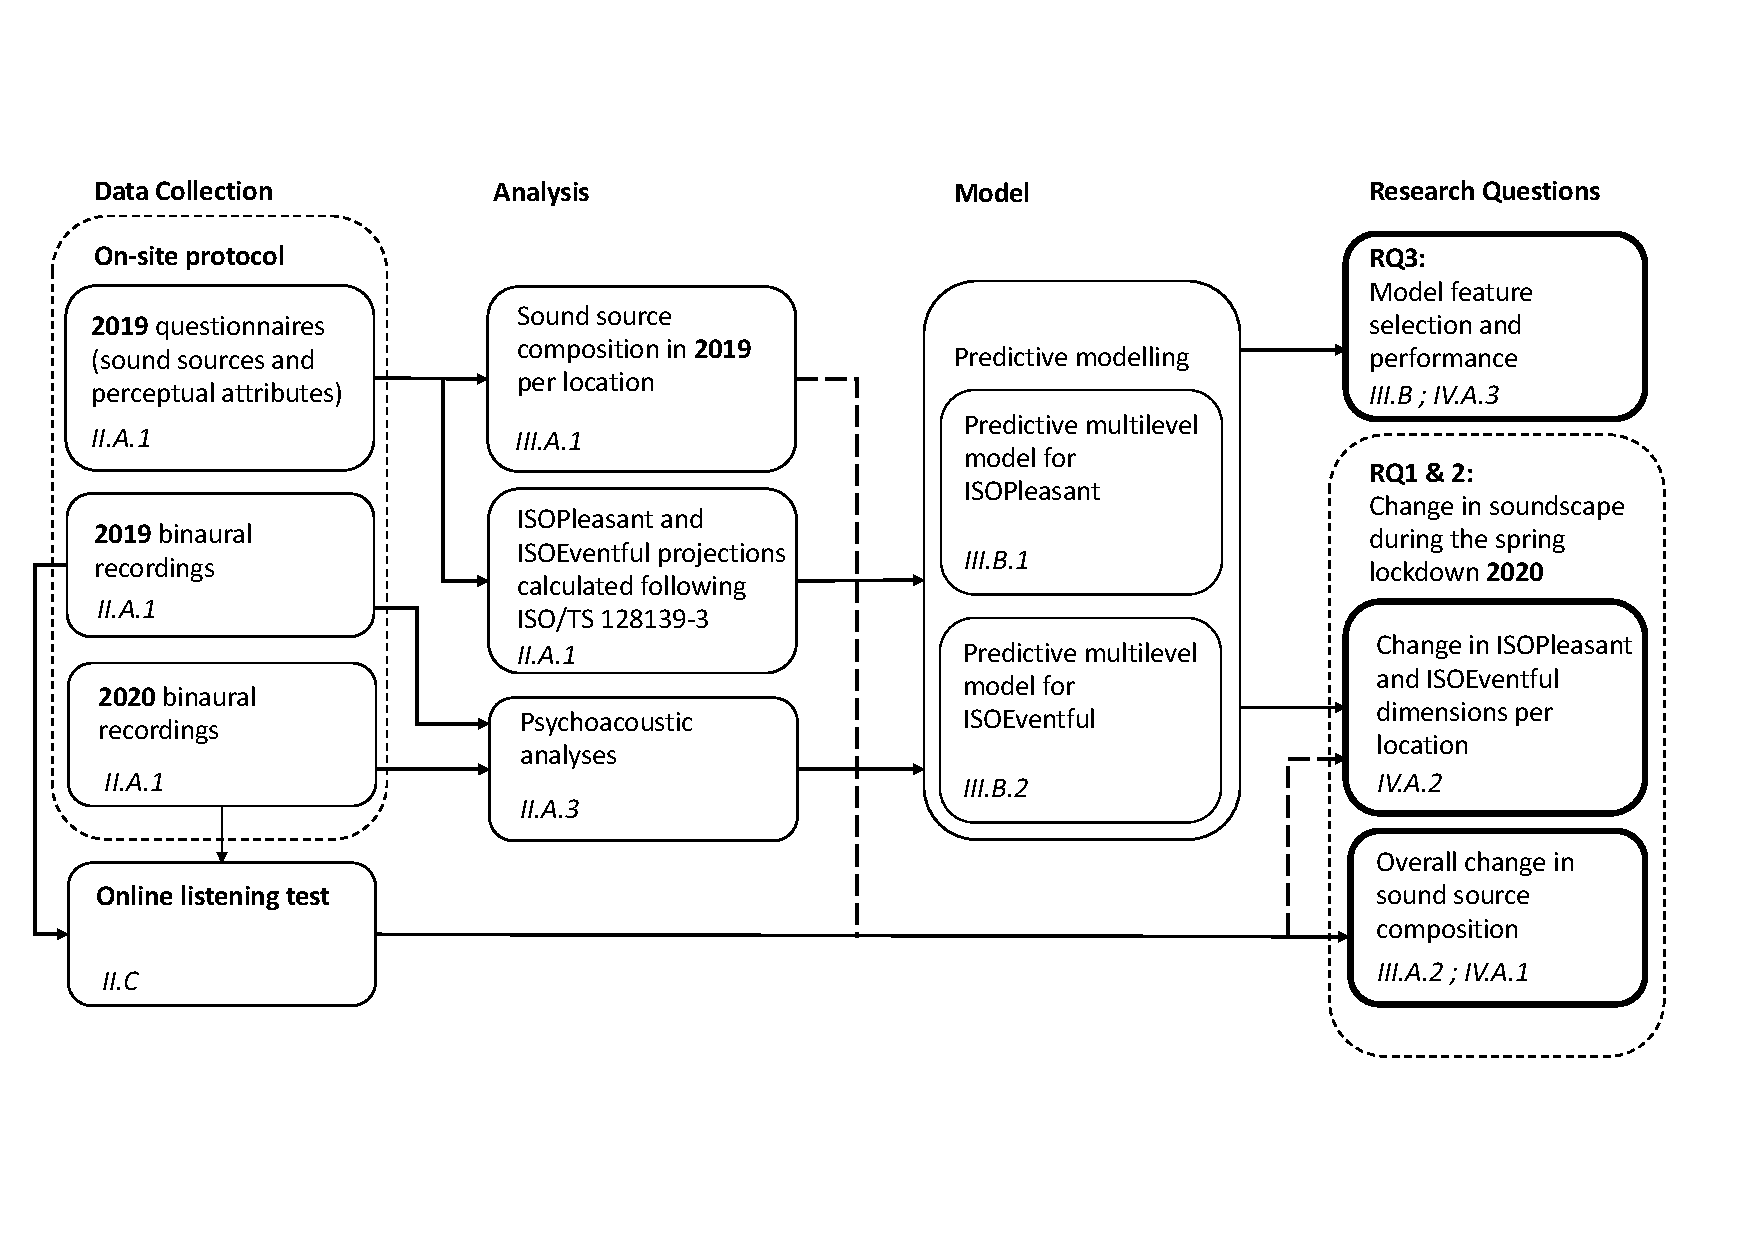
\includegraphics[width=\textwidth]{Figures/Lockdown-Fig1.pdf}
     \caption{The study flowchart indicating the data collection, analysis, modelling, and discussion throughout the study. The subsections in the text to which each box refers are indicated in italics.}
     %FIXME: Change the section references to match.
   \end{figure}

\section{Results}

 The results of the onsite surveys, online experiment, and the model development are reported here. They are reported following the structure of the ISO/TS 12913 series, revealing the perceived sound source dominance, key perceptual attributes (\gls{isopl} and \gls{isoev}) and the lockdown-related changes.

 \subsection{Perceived sound source dominance}

   \subsubsection{2019 sound source composition per location}

   Questionnaire data was collected English, Italian, and Spanish in both cities. The respective questionnaires can be found in the supplementary files and \citet{Mitchell2020Soundscape}. Data presented here was aggregated per LocationID.

   According to the highest scored mean value of the dominant sound source type, as show in Figure \ref{fig:sound-source-dom}, the locations can be grouped into: natural sounds dominated (RegentsParkJapan, RegentsParkFields, RussellSq), human sounds dominated (SanMarco, TateModern, StPaulsRow, StPaulsCross, MonumentoGaribaldi), noise (traffic and other noise) sounds dominated (CamdenTown, EustonTap, TorringtonSq, PancrasLock).

   \begin{figure}
     \label{fig:sound-source-dom}
     \centering
     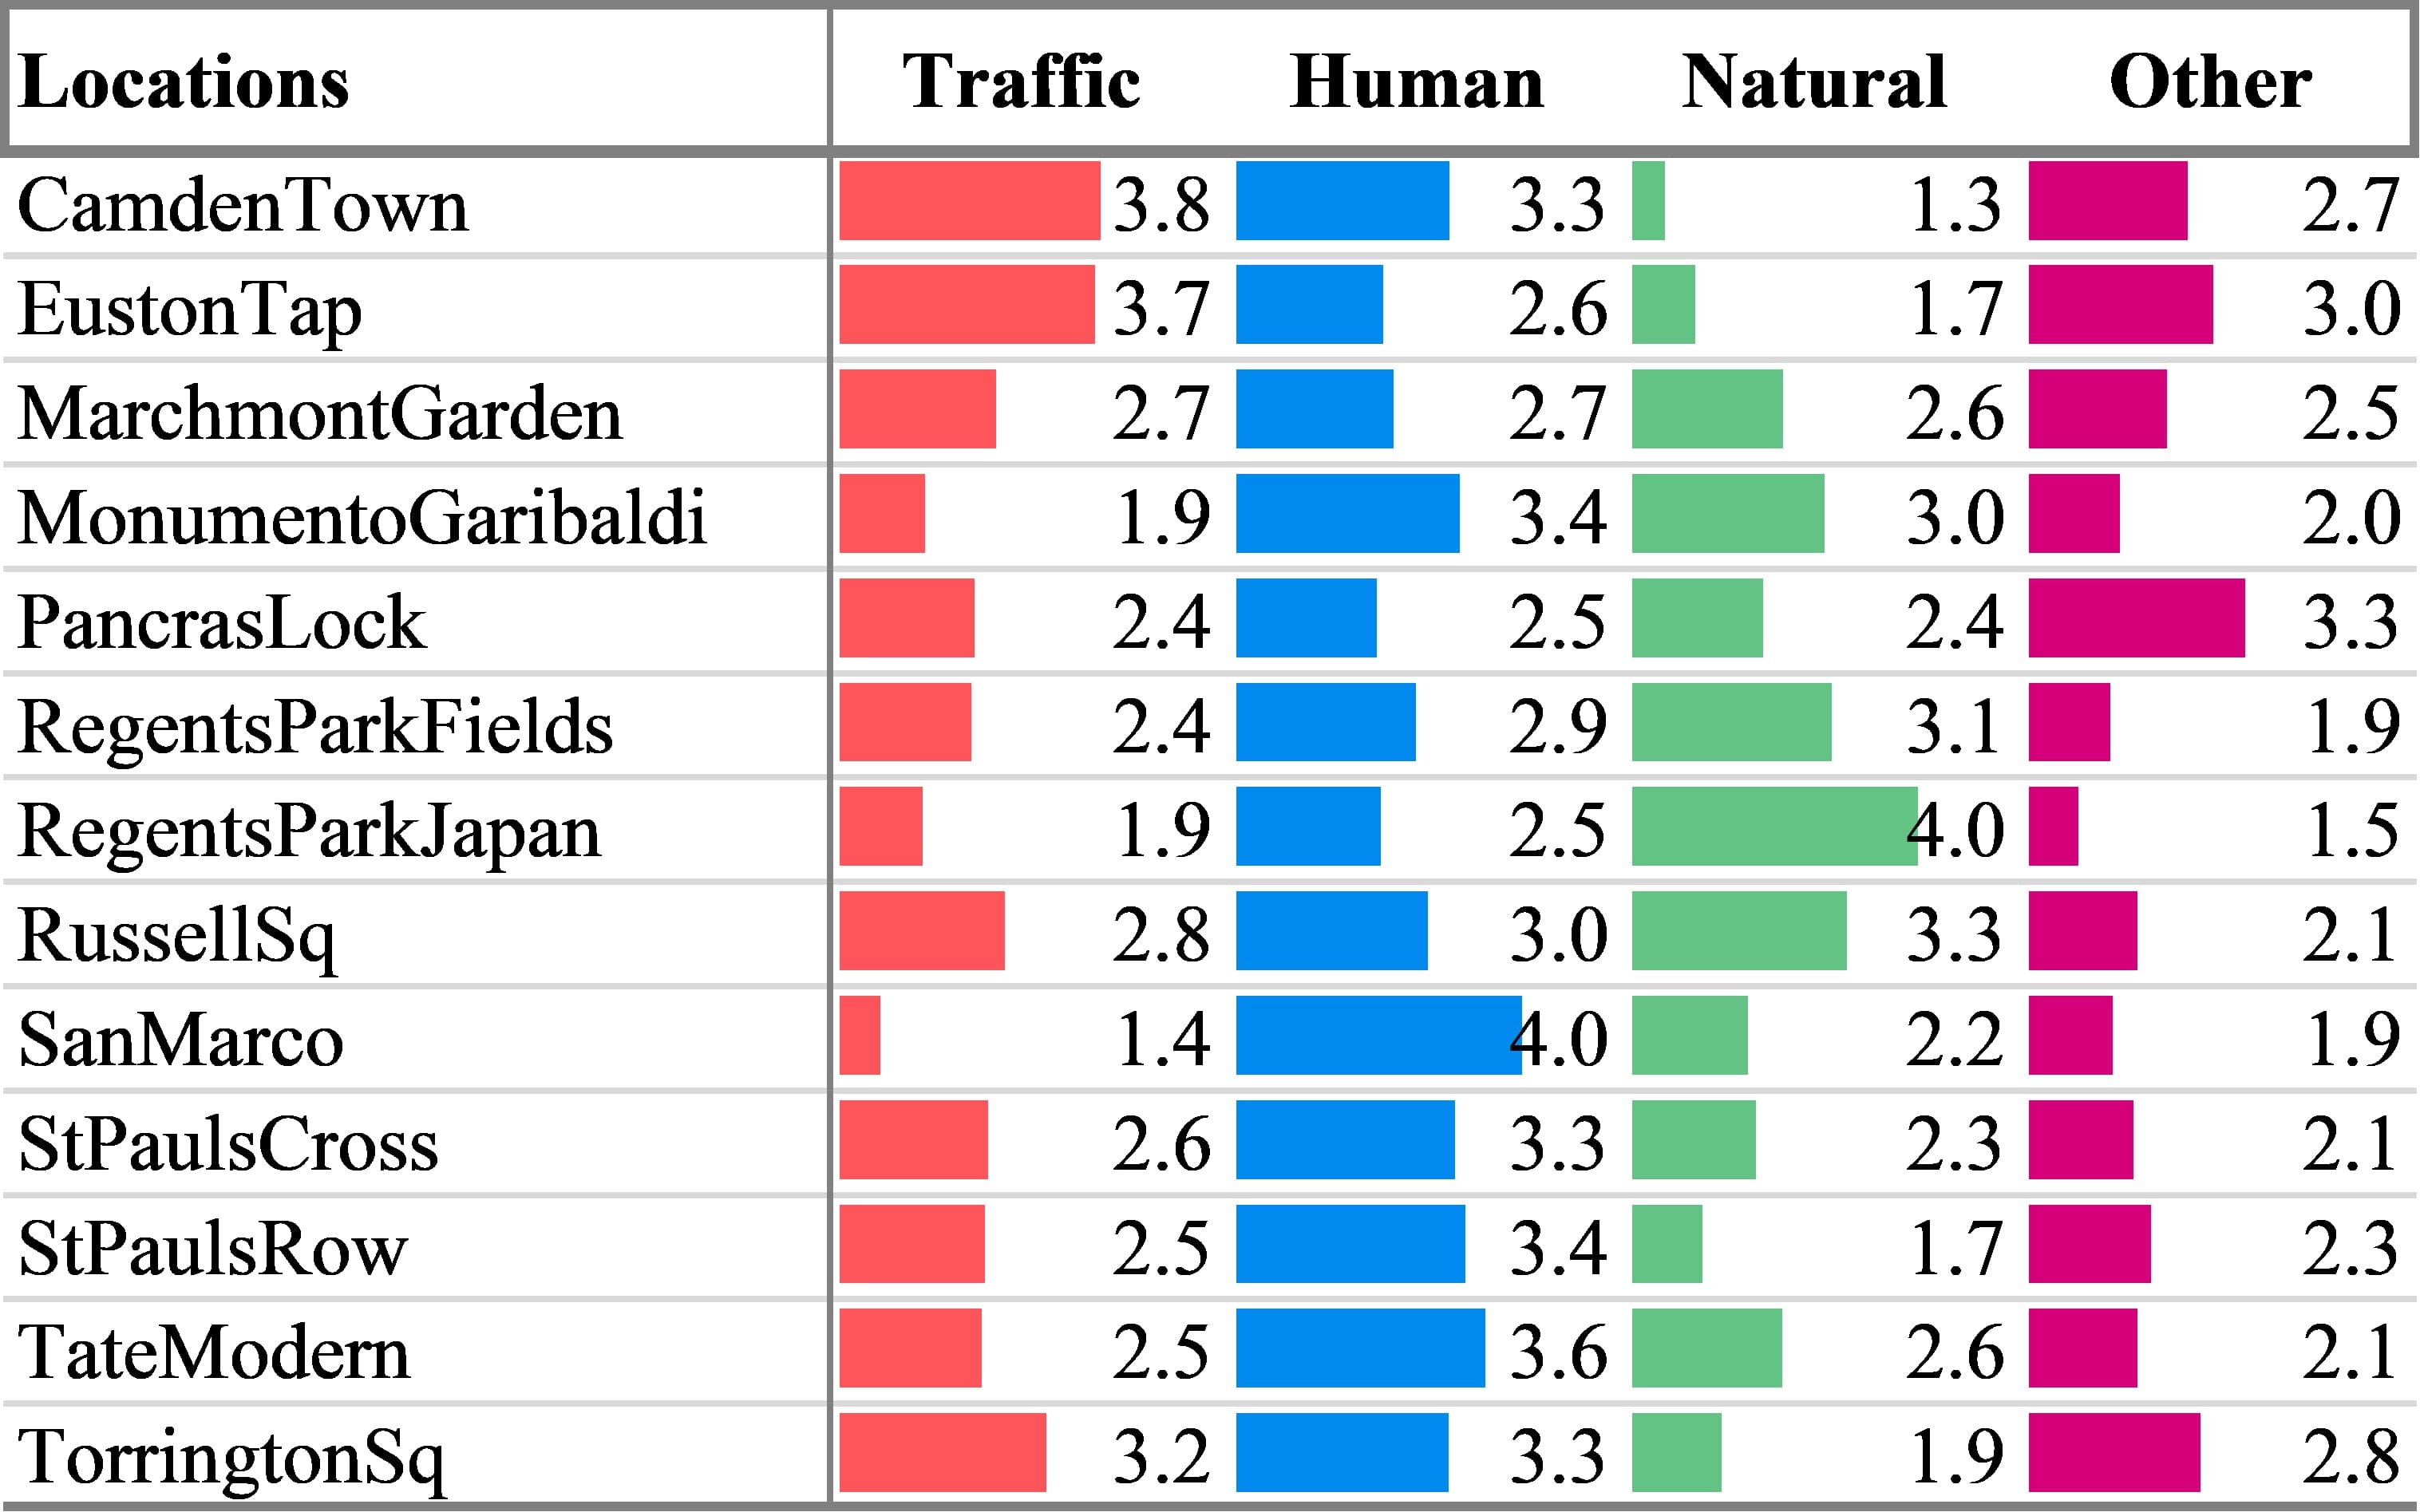
\includegraphics[width=.8\textwidth]{Figures/Lockdown-Fig2.jpg}
     \caption{Mean values per LocationID for the perceived dominance of the sound source types, for the 2019 on-site campaign.}
   \end{figure}

   \subsubsection{Overall change in the perceived sound source dominance during lockdown}

   1,803 words describing the sound sources present in the 2019 recordings and 1,395 words related to the 2020 recordings were input by participants in response to the open-ended question Q1 \draft{(see Appendix A)}. The frequency of occurrence, generated using the Word-Clouds web app, is shown in Figure \ref{fig:wordclouds}, for the 2019 and the 2020 sets respectively. The most frequency words from both 2019 and 2020 groups are: noise, car/traffic, bird/birds, talk/voice, and (foot)steps.

   \begin{figure}
     \label{fig:wordclouds}
     %TODO: add wordcloud figure
   \end{figure}

   The results from the listening tests deployed online were analysed using SPSS Statistics v. 25. Levene's test for equality of variances resulted in highly statistically significant values for all 4 sound sources investigated ($<0.001$). Therefore, a Mann-Whitney U-test was used as a non-parametric equivalent to the t-test to investigate the change in the perceived dominance of the four sound source types \citep{McKnight2010Mann}. The results for human sounds indicated that the perceived dominance was greater for the 2019 sample ($M=3.82$) than for the 2020 sample ($M=2.62, U=41,656, p<0.001$). The results for natural sounds indicated the perceived dominance increased from 2019 ($M=2.00$) to 2020 ($M=2.54, U=63,797, p<0.001$). However, the differences for the noise sources (traffic and other) were not statistically significant.

   \begin{figure}
     \label{tab:source-dominance-stats}
   \end{figure}

 \subsection{Model selection, performance, and application}

   \subsubsection{\gls{isopl} model selected}

   Following the feature selection, the \gls{isopl} model (given in Table \ref{tab:scaled-model}) has \gls{n5} as the fixed effect with a scaled coefficient of -0.06, and \gls{laeq}, \gls{la10la90}, and \gls{lcla} as coefficients which vary depending on the LocationID. The training and testing \gls{mae} are very similar, indicating that the model is neither over- nor under-fitting to the training data ($MAE_{train}=0.259, MAE_{test}=0.259$). The model performs very well at predicting the average soundscape assessment of the locations ($R^2_{train}=0.998, R^2_{test}=0.85$).

  %FIXME: fix layout of model table
   \begin{table}[ht]
    \label[]{tab:scaled-model}
  \centering
\caption{Scaled linear regression models of \gls{isopl} and \gls{isoev} for 13 locations in London and Venice. The \gls{isopl} model is a multi-level regression model with one level for individual effects and a second level for LocationID effects, while the \gls{isoev} model is a 'flat' multi-variate linear regression with no location effects.}
  \label{tab:model}

  \def\arraystretch{.5}
  \begin{tabular}{@{}l|lccccc@{}}
    \toprule
    \multicolumn{1}{l|}{}                    &
    \multicolumn{3}{c}{\textbf{ISOPleasant}} &
    \multicolumn{3}{c}{\textbf{ISOEventful}}                                                                                                                                                           \\
    \textit{Predictors}                      &
    \multicolumn{1}{c}{\textit{Estimates}}   &
    \textit{CI}                              &
    \textit{p}                               &
    \textit{Estimates}                       &
    \textit{CI}                              &
    \textit{p}                                                                                                                                                                                         \\ \midrule
    (Intercept)                              &
    \multicolumn{1}{c}{0.24}                 &
    0.15 - 0.33                              &
    \textbf{\textless{}0.001}                &
    0.14                                     &
    0.12 - 0.16                              &
    \textbf{\textless{}0.001}                                                                                                                                                                          \\
    $N_5$                                    & \multicolumn{1}{c}{-0.06}                               & -0.10 - -0.02 & \textbf{\textless{}0.001} &       &               &                           \\
    S                                        & \multicolumn{1}{c}{}                                    &               &                           & -0.08 & -0.11 - -0.06 & \textbf{\textless{}0.001} \\
    FS                                       & \multicolumn{1}{c}{}                                    &               &                           & -0.02 & -0.05 - -0.00 & \textbf{0.033}            \\
    T                                        & \multicolumn{1}{c}{}                                    &               &                           & 0.04  & 0.01 - 0.07   & \textbf{0.002}            \\
    $L_{Aeq}$                                & \multicolumn{1}{c}{}                                    &               &                           & 0.14  & 0.11 - 0.17   & \textbf{\textless{}0.001} \\
    $L_{Ceq}-L_{Aeq}$                        & \multicolumn{1}{c}{}                                    &               &                           & -0.03 & -0.05 - 0.00  & 0.052                     \\
    \\
    \textbf{Random Effects}                  &
                                             &
    \multicolumn{1}{l}{}                     &
    \multicolumn{1}{l}{}                     &
    \multicolumn{1}{l}{}                     &
    \multicolumn{1}{l}{}                     &
    \multicolumn{1}{l}{}                                                                                                                                                                               \\
    $\sigma^2$                               &
    0.11                                     &
    \multicolumn{1}{l}{}                     &
    \multicolumn{1}{l}{}                     &
    \multicolumn{1}{l}{}                     &
    \multicolumn{1}{l}{}                     &
    \multicolumn{1}{l}{}                                                                                                                                                                               \\
    $\tau_{00}$                              & \multicolumn{6}{l}{$0.03_{LocationID}$}                                                                                                                 \\
    $\tau_{11}$                              & \multicolumn{6}{l}{$0.02_{LocationID.L_{Aeq}}$}                                                                                                         \\
                                             & \multicolumn{6}{l}{$0.00_{LocationID.L_{A10}-L_{A90}}$}                                                                                                 \\
                                             & \multicolumn{6}{l}{$0.00_{LocationID.L_{Ceq}-L_{Aeq}}$}                                                                                                 \\
    ICC                                      &
    0.90                                     &
    \multicolumn{1}{l}{}                     &
    \multicolumn{1}{l}{}                     &
    \multicolumn{1}{l}{}                     &
    \multicolumn{1}{l}{}                     &
    \multicolumn{1}{l}{}                                                                                                                                                                               \\ \midrule
    N                                        & \multicolumn{6}{l}{$13_{LocationID}$}                                                                                                                   \\
    Observations                             &
    914                                      &
    \multicolumn{1}{l}{}                     &
    \multicolumn{1}{l}{}                     &
    \multicolumn{1}{l}{914}                  &
    \multicolumn{1}{l}{}                     &
    \multicolumn{1}{l}{}                                                                                                                                                                               \\

    MAE Test, Train                          &
    0.258                                    &
    0.259                                    &
                                             &
    \multicolumn{1}{l}{0.233}                &
    0.231                                                                                                                                                                                              \\

    \bottomrule
  \end{tabular}
\end{table}

   The high intraclass correlation ($ICC=0.90$) demonstrates that the location-level effects are highly important in predicting the pleasantness dimension. Within this random-intercept random-slope model structure, these effects include both the specific context of the location (i.e. the LocationID factor), but also the \gls{laeq}, \gls{la10la90}, and \gls{lcla} features whose effects vary across locations. These slopes are given in Figure \ref{fig:pl-slopes}. This point highlights the need to consider how the context of a location will influence the relationship between the acoustic features and the perceived pleasantness.

   \begin{figure}
     \label{fig:pl-slopes}
     \caption{Location-level scaled coefficients for the \gls{isopl} model.}
     \centering
     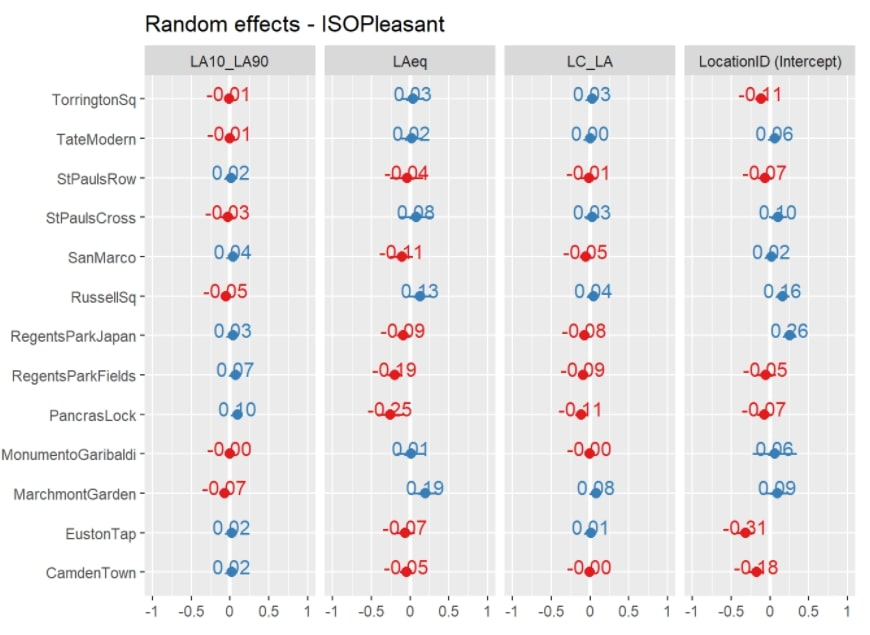
\includegraphics[width=\textwidth]{Figures/Lockdown Figure4.jpg}
   \end{figure}

   \subsubsection{\gls{isoev} model selected}

   Through the group-level feature selection, all of the group-level coefficients, including the LocationID factor itself. Therefore the final \gls{isoev} model is a 'flat' multi-variate linear regression model, rather than a multi-level model. The \gls{isoev} is a linear combination of \gls{s}, \gls{fs}, \gls{tu}, \gls{laeq}, and \gls{lcla}. The training and testing \gls{mae} are very similar, indicating that the model is not over-fit to the training data ($MAE_{train}=0.233; MAE_{test}=0.231$). The model performs slightly worse than the \gls{isopl} at predicting the mean location responses, but still performs well ($R^2_{train}=0.873; R^2_{test}=0.715$).

   \subsubsection{Application to lockdown data}
   %FIXME: Figure out how to do sub-figure referencing
   Once the two models were built and assessed, they were then applied to the lockdown recording data in order to predict the new soundscape ISO coordinates. Figure \ref{fig:circumplex-locations}(a) shows the pre-lockdown ISO coordinates for each location and Figure \ref{fig:circumplex-locations}(b) shows how the soundscapes are predicted to have been assessed during the lockdown period. As in the model assessment process, the predicted responses are calculated for each recording individually, then the mean for each location is calculated and plotted on the circumplex.

   In 2019 the majority of locations in the dataset fall within the 'vibrant' quadrant of the circumplex, particularly those which are primarily dominated by human activity (e.g. SanMarco, TateModern). CamdenTown and EustonTap, which are both in general visually and acoustically dominated by traffic, are the only two to be rated as 'chaotic', while no locations are overall considered to be 'monotonous'. During the 2020 lockdown, there is a general positive move along the 'pleasant' dimension and a general negative move along the 'eventful' dimension, but several patterns of movement can be noted. These are investigated further in the Discussion section below.

   \begin{figure}
     \label{fig:circumplex-locations}
     \caption{Soundscape circumplex coordinates for (a) the mean \gls{isopl} and \gls{isoev} responses for each location; and (b) the mean predicted responses based on recordings made during the lockdown and the location's movement in the circumplex.}
     \centering
     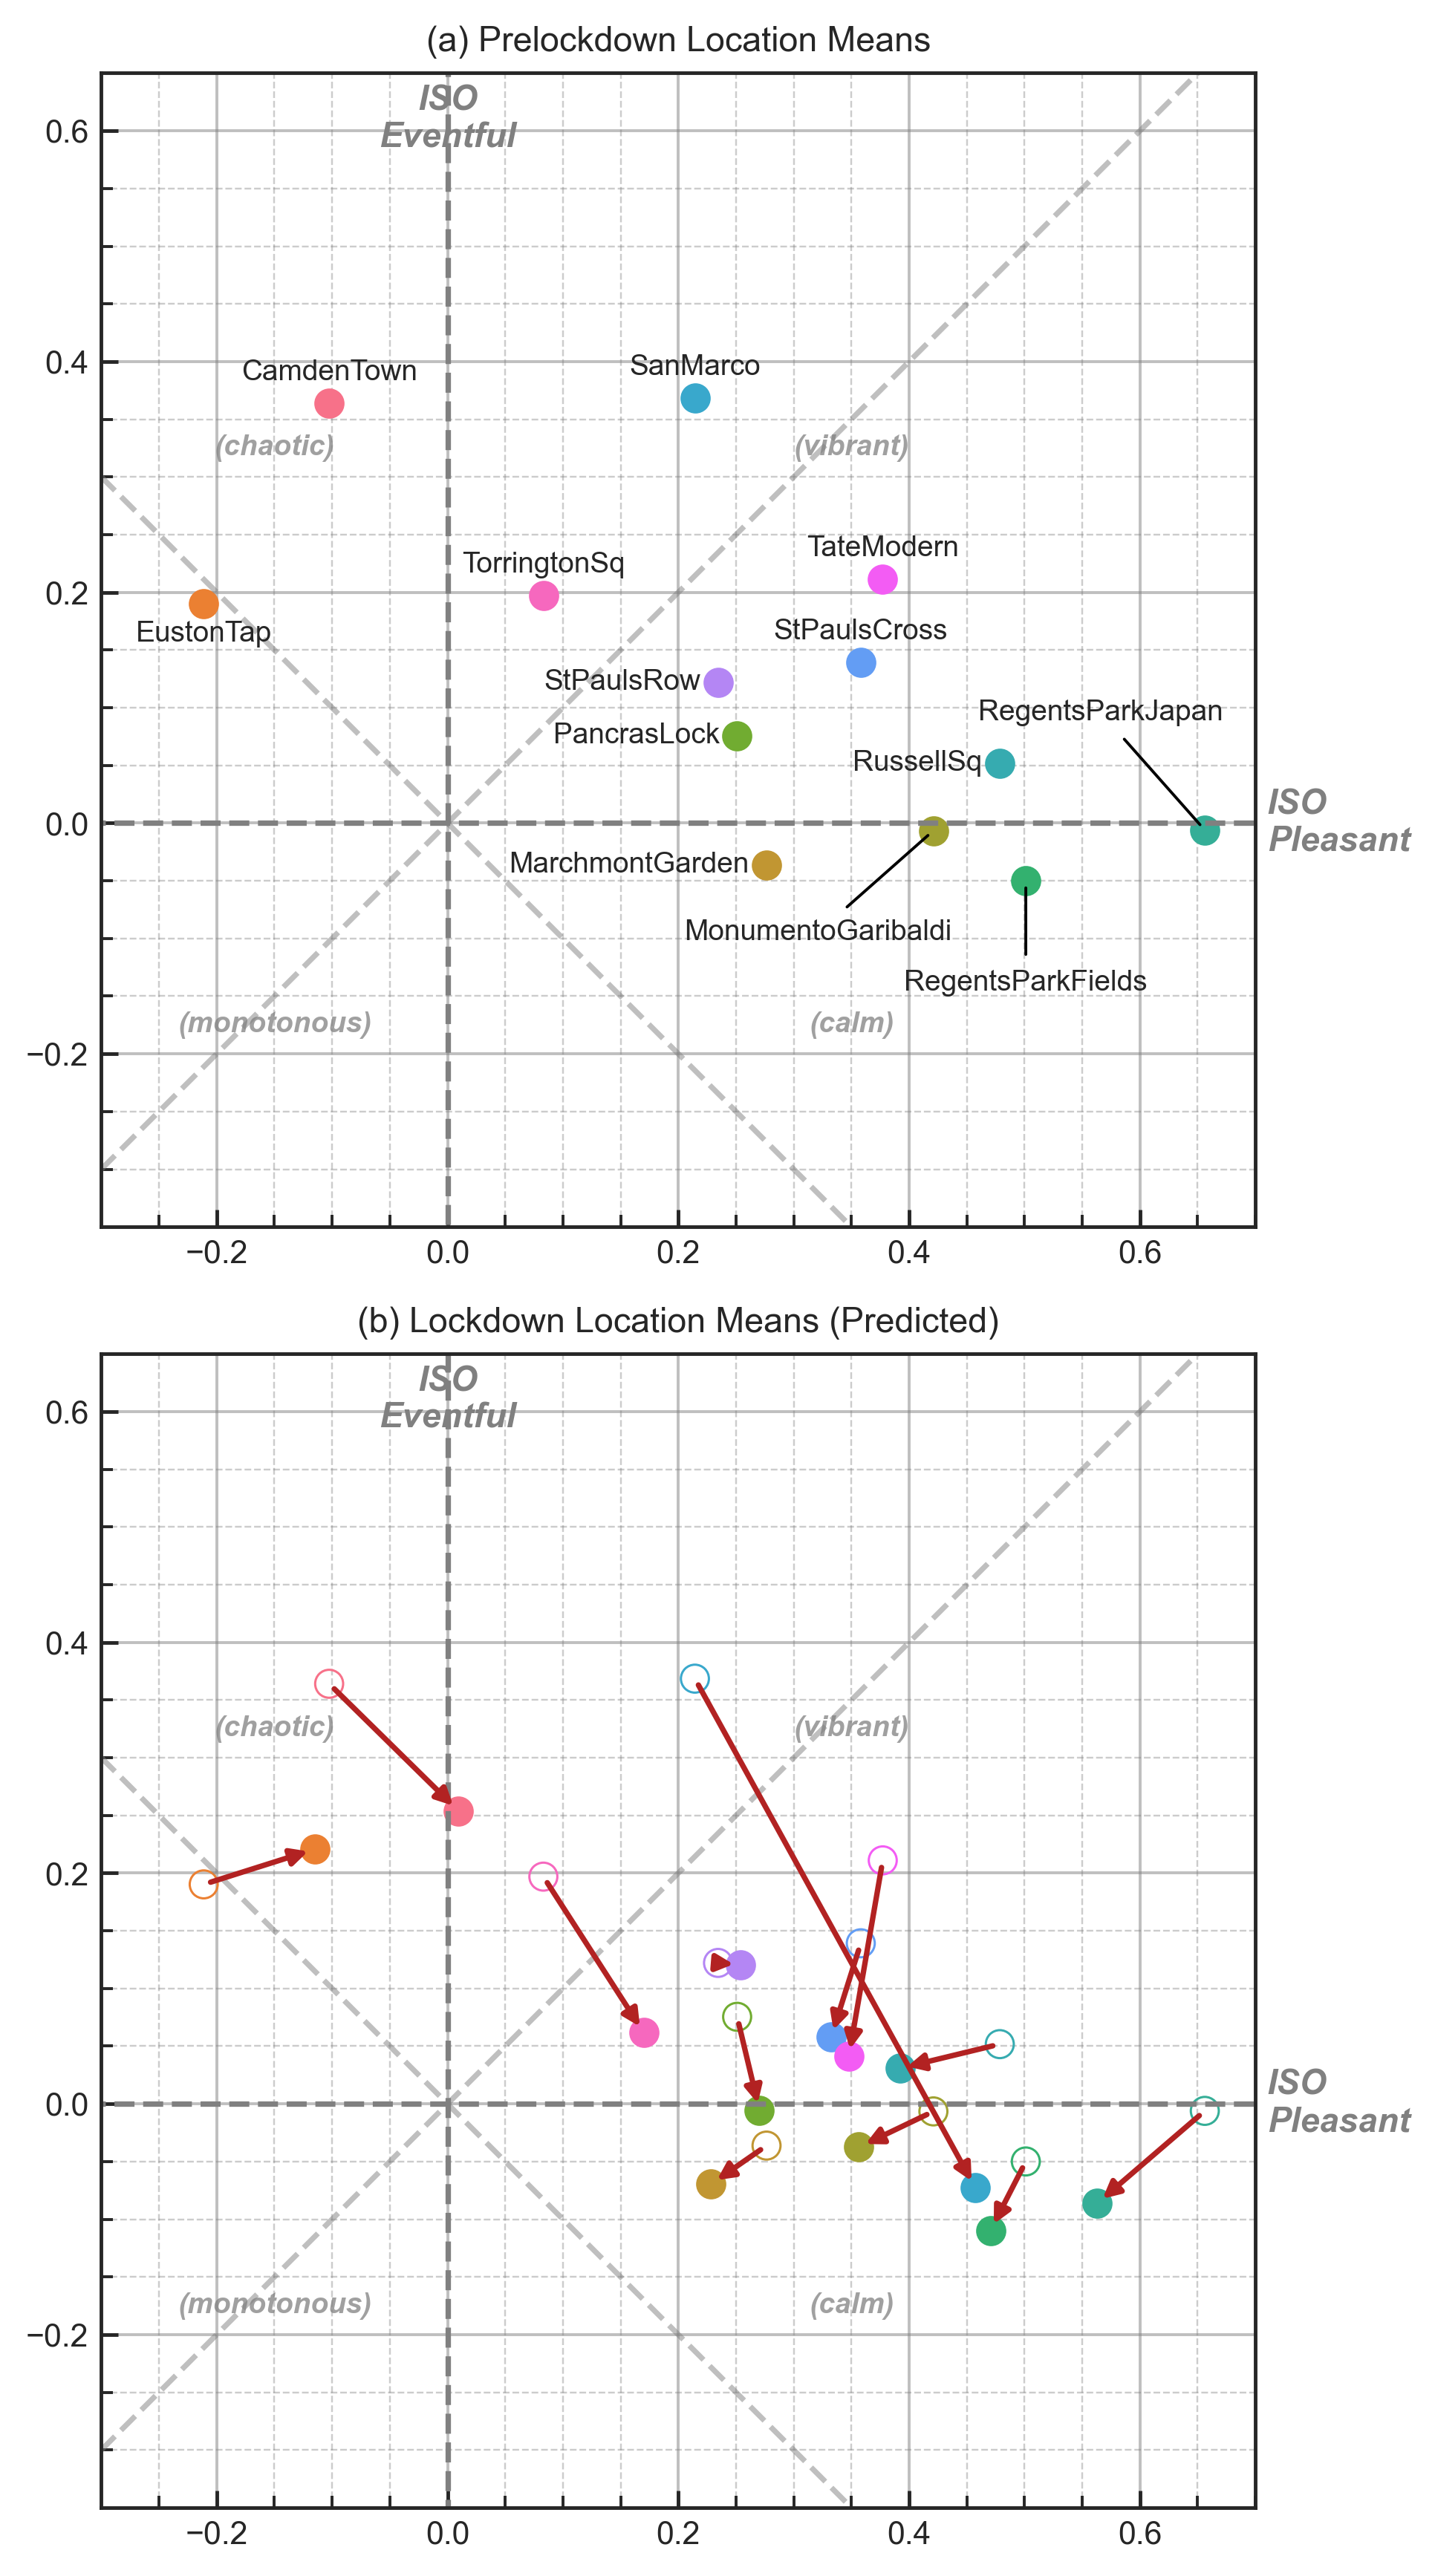
\includegraphics[width=.75\textwidth]{Figures/Lockdown Figure5.jpg}
   \end{figure}

   %%%%%%%%%%%%%%%%%%%%%%%%%%%%%%%%%%%%%%%%%%%%%%%%%%%%%%%%%%%

\section{Discussion}

 \subsection{Interpretation of the results}

   To interpret the results addressing RQ1 and RQ2, it is necessary to separately look into the overall change in sound source composition, and the change in the affective quality of soundscapes per location.

   \subsubsection{Change in the sound source composition}

   The open-ended question about sound sources in the online survey did not reveal a change in sound source types but rather confirmed that all types were still present in both conditions. The sound source composition question taken from the Method A of the ISO/TS 12913-2:2018 \citep{ISO12913_2_2018IOS} revealed a statistically significant reduction in human sound sources and a significant increase in the perceived dominance of natural sound sources.

   The most frequent sound sources detected from the open-ended question correspond to the main four sound source types investigated, which indicated that all types remained present in the lockdown condition (at all the locations). While traffic intensity might have gone down, where the results of the Mann-Whitney U-test were inconclusive, but supported by the psychoacoustic measurements according to \citet{Aletta2020Assessing}, traffic-related sound sources were still clearly present.

   The sound source composition of an outdoor acoustic environment is extremely complex. Removing one component, such as human sounds, has implications on the whole \citep{Gordo2021Rapid}. Testing the effects of this in-situ is not straightforward and interpreting this study in line with 'what is the impact of human sounds' must be taken within the broader context of the range of conditions which changed within the acoustic environment. However, looking at the overarching picture, the lockdown condition was a useful and unique case study to understand the impact which human activities -- and the human sound source type in particular -- can have on soundscape perception of urban open spaces.

   \subsubsection{Movement of soundscapes}

   In order to interpret how the change of the acoustic environment at the locations examined would have been perceived, and to answer RQ2, movement vectors within the circumplex space are shown in Figure \ref{fig:circumplex-vectors}. This clearly shows a few different patterns of movement due to the effects of the 2020 lockdown. These can be further looked into depending:

   \begin{enumerate}
     \item the magnitude of change,
     \item the direction of change,
     \item shift between the quadrants shown in Figure \ref{fig:circumplex-locations},
     \item sound source composition.
   \end{enumerate}

   \begin{figure}
     \label{fig:circumplex-vectors}
     \caption{The relative movement of soundscape perception in the circumplex due to the \gls{covid19} lockdowns, represented as vectors centred on the origin. *The lawn-works dominated session is shown separately as MonumentoGaribaldi* with a grey arrow to indicate that this is distinct from the effects of the lockdown changes.}
    \centering
    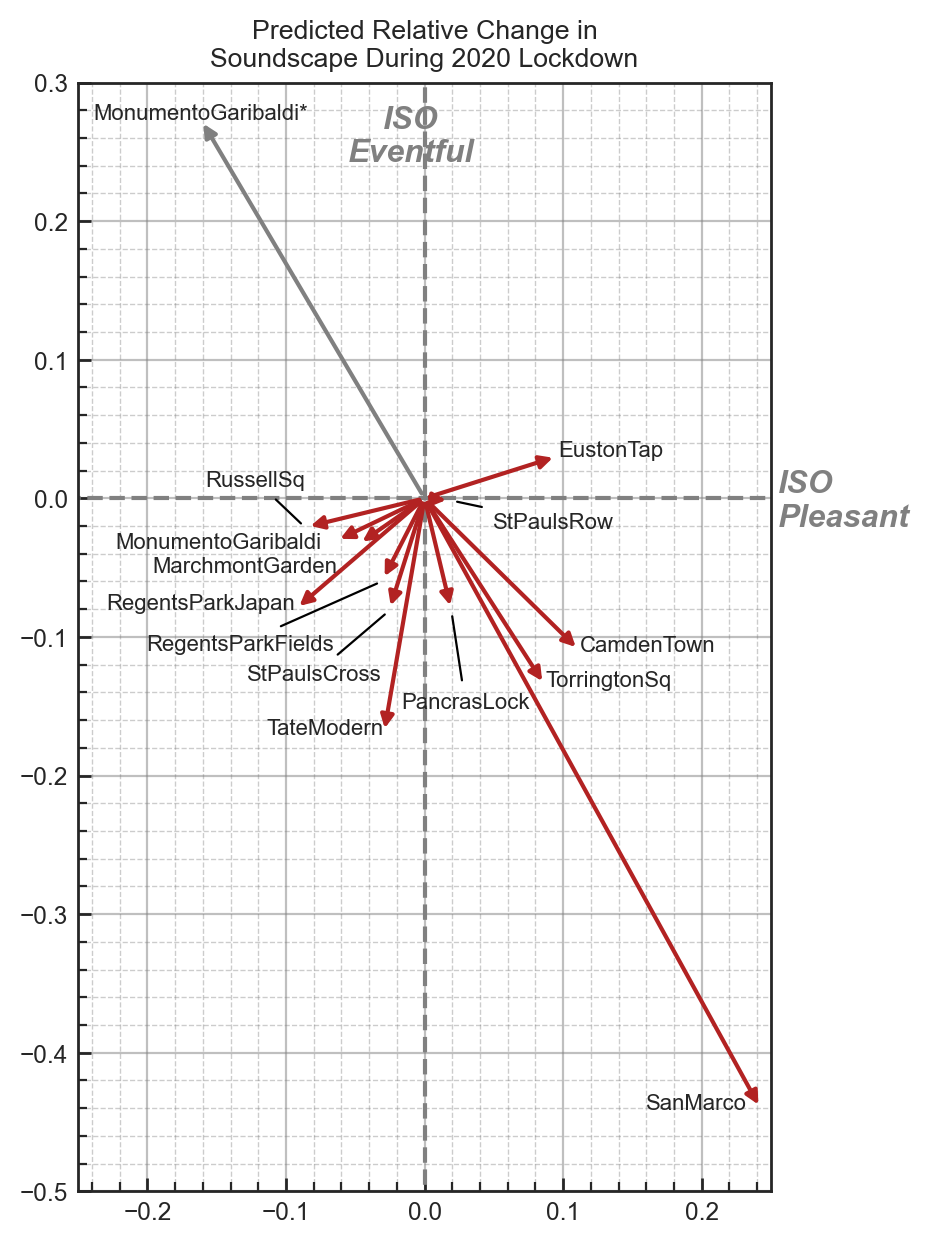
\includegraphics[width=.75\textwidth]{Figures/Lockdown Figure6.jpg}
   \end{figure}

   \paragraph{SanMarco} The largest change is seen in Piazza San Marco, with a predicted increase in pleasantness of 0.24 and a decrease in eventfulness of 0.44, enough to move the soundscape out of the 'vibrant' quadrant and into 'calm'. This extreme change (relative to the rest of the locations) is exactly what would be expected given the unique context of the measurements taken in 2019 -- the measurement campaign corresponded with Carnevale, a yearly festival which centres around the square. By contrast, due to the particularly strict measures imposed in Italy, during the lockdown measurement period the square was almost entirely devoid of people. What is promising is that, without any of this contextual information about the presence or absence of people, our model is able to capture and reflect what may be considered a reasonable and expected direction and scale of movement within the soundscape circumplex.

   \paragraph{EustonTap, CamdenTown, TorringtonSq, PancrasLock} The next locations of interest are those which, in the 2019 survey data, were rated as being dominated by traffic noise: EustonTap, CamdenTown, TorringtonSq, and PancrasLock. These are the only locations (besides SanMarco) which show a predicted increase in pleasantness. Of these traffic-dominated spaces, the two which were most heavily dominated by traffic noise (CamdenTown and EustonTap) showed the most increase in pleasantness, with TorringtonSq having slightly less of an increase. PancrasLock, which was also rated as having high levels of both Human and Natural sounds shows only a modest improvement in pleasantness.

   \paragraph{StPaulsCross, TateModern, RegentsParkJapan, RegentsParkFields, RussellSq} Among the locations which are predicted to experience a negative effect on pleasantness we see a mix of spaces which were assessed as being dominated by Human (StPaulsCross and TateModern) and Natural (RegentsParkJapan, RegentsParkFields, RussellSq) sounds before the lockdown. It is hard to discern a pattern of difference between these two groups, although it appears that the Human-dominated spaces saw a greater reduction in eventfulness, compared to the Natural-dominated spaces.

   In general, we note that most of the spaces experience some degree of reduction in eventfulness. This pattern is particularly consistent with what would be expected from a reduction in human presence in these spaces \citep{Aletta2018Towards}, as reflected by the observation that, in general, those spaces which had the most human sounds prior to the lockdown showed the greatest reduction in eventfulness during the lockdown.

   \paragraph{EustonTap} An unexpected result is that EustonTap is predicted to experience an increase in eventfulness and it is unclear whether this accurately reflects the real experience people would have had in the space. Normally, EustonTap is a mostly-outdoor drinking venue located at the entrance to the Euston Train station and is situated directly along a very busy central London road. During the 2020 survey, the researchers noted that the music and chatter of people from the pub was noticeably missing, but that the perceived reduction in road traffic was minimal. Based on the theory of vibrancy which would suggest it is driven by human presence and sounds \citep{Aletta2018Towards}, we would not therefore expect a shift in the vibrant direction as indicated here. This discrepancy may reveal a weakness in the context-independent \gls{isoev} model, or it may in fact be indicating that, at certain thresholds of traffic noise, a reduction in level -- and therefore a reduction in energetic masking -- will allow other aspects of the sound to influence the perception.

   \paragraph{MonumentoGaribaldi} Finally, special attention should be paid to the results shown for Monumento Garibaldi, which in 2019 was perceived as a pleasant and slightly calm green space featuring a gravel walkway. During the first measurement session during the lockdown in 2020, the researcher noted that the soundscape was dominated by landscaping works, in particular noise from strimmers (or weed whackers). In order to gain a sample which was more representative of the impact of the lockdowns, the researcher returned another day to repeat the measurements without interference from the works.

   To examine the impact of these two scenarios separately, the prediction model was fitted to the data from the two sessions independently and the session which was impacted by the landscaping works is shown in Figure \ref{fig:circumplex-vectors} in grey and labelled MonumentoGaribaldi*, while the unaffected session is shown in red. In the latter case, the predicted change in soundscape as a result of the lockdowns fits neatly into what would be expected can closely matches the predicted behaviour of similar locations in London (i.e. MarchmontGarden and RussellSq). On the other hand, the session which was dominated by noise from the strimmers is predicted to have become much more chaotic, with a decrease in pleasantness of 0.16 and an increase in eventfulness of 0.27. This indicates that, although the model has no contextual information about the type of sound and in fact the training data never included sounds from similar equipment, just based on the psychoacoustic features of the sound it is able to reasonably predicted the expected change in soundscape.

   \paragraph*{}As a whole, the primary impact of the 2020 lockdowns on the soundscapes in London and Venice was an overall decrease in eventfulness. With the exception of EustonTap, all of the sessions show some degree of reduction in eventfulness, reflecting the general decrease in sound levels and human sound sources across the locations. The impact of the lockdowns on pleasantness is more mixed and seems to be driven by the previous dominance of traffic noise in the space. However, it could also be noted that, while all locations experienced a reduction in sound level, those which are predicted to become more pleasant had an average \gls{laeq} above 60 dB in 2019. By contrast, the locations which were predicted to experience a decrease in pleasantness generally had sound levels below 60 dB(A) in 2019. This may indicate that reductions in sound level can improve pleasantness when the sound level exceeds some threshold of around 60 - 65 dB(A) but are ineffective when sound levels are below this threshold. Similarly, \citet{Yang2005Acoustic} showed that, when the sound level is 'lower than a certain a certain value, say 70 dB' there is no longer a significant improvement in the evaluation of acoustic comfort as the sound level reduces. It is unclear at this point where this threshold would lie for pleasantness/annoyance, how strict it may be, or how it is impacted by the sound source composition of the acoustic environment, therefore further research is needed in this area.

   \subsubsection{Model selection results}

   The most immediately interesting result of the model-building and feature selection process, answering to RQ3, is the apparent irrelevance of location context to the \gls{isoev} dimension. The multilevel model structure was chosen since the starting assumption was that soundscape perception is heavily influenced by contextual factors, such as expectations of the space and visual context \cit{add references}. For this modelling, these factors can be considered as location-level latent variables at least partially accounted for by the inclusion of the LocationID as the second-level factor. While this assumption certainly held true for \gls{isopl}, our results indicate that these types of contextual factors are not significant for \gls{isoev}, and do not affect the relationship between the acoustic features of the sound and the perception.

   In particular this result may herald a shift in modelling approach for soundscapes -- where previous methods, in both the soundscape and noise paradigms, have mostly focused on deriving acoustic models of annoyance (in other words have focussed on the \gls{isopl} dimension) perhaps they should instead consider the acoustic models as primarily describing the eventfulness dimension when considered in-situ. In addition this study takes the approach of modelling responses at an individual level in order to derive the soundscape assessment of the location. Rather than either attempting to represent the predicted response of an individual person -- which is less useful in this sort of practical application -- or to base the model on average metrics of the location, the goal is instead to characterise the location itself, through the aggregated predicted responses of individuals. The authors believe this modelling approach better addresses the practical goal of predictive soundscape modelling and reflects the structure of the data collection.

   %TODO: Expand on this concept for the thesis.

 \subsection{Limitations of the study}

   The onsite sampling method was initially not intended as the ultimate characterisation of a location's soundscape but rather as a tool for model development. Therefore, the change observed does not necessarily represent the ground truth about the site's soundscape, if such a thing exists. Further, the online listening tests took a relatively small but random sample from the available database and did not include any contextual information. This proved to be sufficient for the purpose of detecting a change in sound source composition, however, the relatively small sample of recordings included in the online study does limit how representative they are of the location's sound environment as a whole.

   The surveys and recordings taken represent only a snapshot of the soundscape or sound environment for a short period in time. This is a flaw in most soundscape sampling methods presented both in the literature and in ISO/TS 12913-2. To truly be said to characterise the soundscape of a space, long-term monitoring and survey methods will need to be developed in order to capture the changing environmental and contextual conditions in the space. Models of the sort presented here, which are based on measurable quantities, could prove to be useful in this sort of long-term monitoring as they could take continuous inputs from sensors and generate the likely soundscape assessment over time.

   Further, the lockdown condition is likely to cause distortions of the circumplex soundscape perception model. Therefore, it is important to acknowledge that all the predictions were made for the people with no experience of the pandemic and its psychological effects. Conceptually, this model captured the perceptual mapping (i.e. the relationship between the acoustic indicator inputs and the soundscape descriptor outputs) of people in 2019, but this perceptual mapping is likely to have been affected by the psychological and contextual impacts of the lockdown itself, independent of its changes on the sound environment. Future research might look into potential perception changes in the post-pandemic world.

   %%%%%%%%%%%%%%%%%%%%%%%%%%%%%%%%%%%%%%%%%%%%%%%%%%%%%%%%%%%%%%%%%%%%%%%%%%

\section{Conclusion}

 This study demonstrates an application of predictive modelling to the field of soundscape studies. The model building results reveal that, within this dataset, an approach based on psychoacoustics can achieve $R^2=0.85$ for predicting the pleasantness of locations and $R^2=0.715$ for predicting the eventfulness. A modelling-focussed method of this sort is a key component to the potential scalability of the soundscape approach to applications such as smart city sensing, urban planning, and cost-effective, sustainable design. To demonstrate the usefulness and feasibility of such an approach, we apply our predictive model to a unique case study in which traditional soundscape survey methods were impossible.

 By applying this predictive model to recordings collected during the 2020 lockdown, the change in perception of the urban soundscapes is revealed. In general, soundscapes became less eventful, and those locations which were previously dominated by traffic noise became more pleasant. By contrast, previously human- and natural-dominated locations are in fact predicted to become less pleasant despite the decrease in sound levels. Although the results are limited in that they present one snapshot of the soundscape of the spaces, the success of the model in responding to new and disturbing sound events demonstrates its potential usefulness in long-term monitoring of urban soundscapes.

 %TODO: Sort out appendix and supplementary material from lockdown paper.